\section{ Applying Linear Combination to Limits }

\displaytwocaption{Results of Using Linear Combination for Limits}{
    The new combination results currently are not using more advanced features of the limit setting framework 
    (NN Background Reweighting or better binning), hence the slightly degraded limits
}{c2v_scan_official}{Original 3 Term Combination}
{c2v_scan_new_kl1.0}{New 6 Term Combination}


\displaythree{$\kvv$ Scans Outside $\kl=1$}
{ Linear combination equation seems to work well beyond the SM value of $\kl$ }
{c2v_scan_scan_test_beta5_samps_vbf_pd_161718_kl1.0_xsec}
{c2v_scan_scan_test_beta5_samps_vbf_pd_161718_kl3.0_xsec}
{c2v_scan_scan_test_beta5_samps_vbf_pd_161718_kl7.0_xsec}

\frame{
    \frametitle{Two Dimensional Exclusion Zone} 
    \begin{columns}
        \begin{column}{0.5\textwidth}
            \begin{figure}
                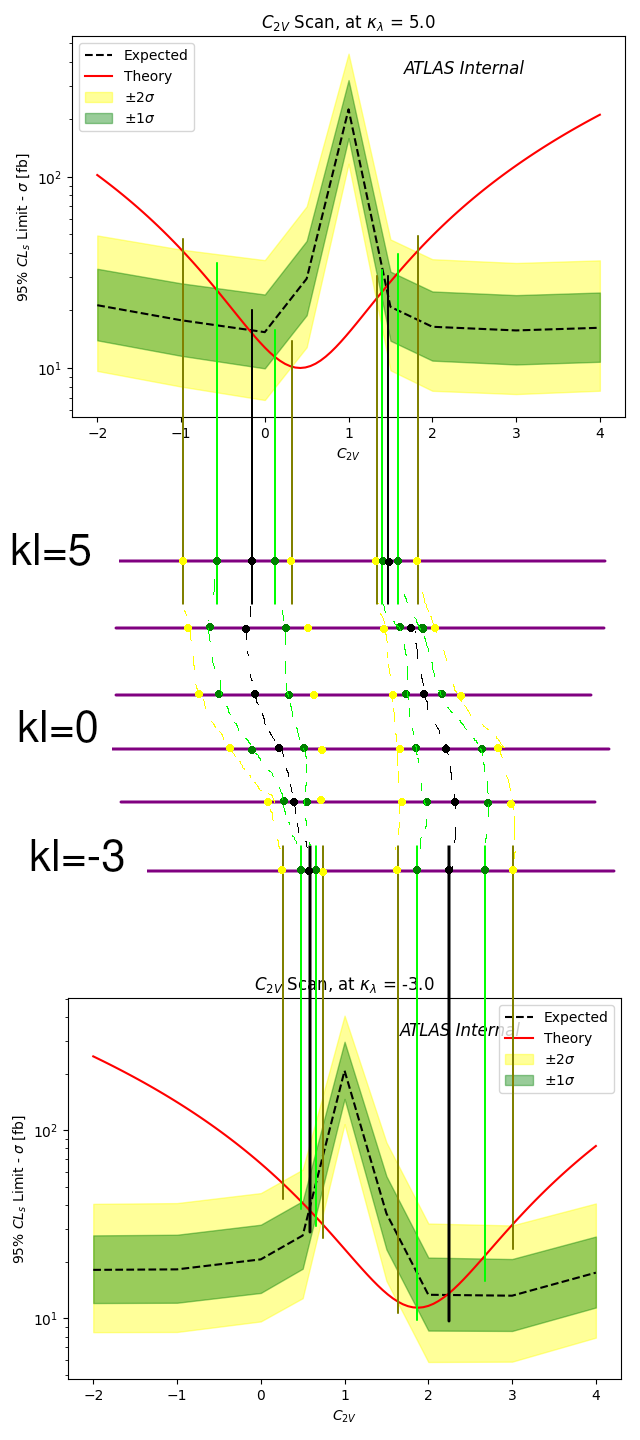
\includegraphics[width=\linewidth,height=0.8\textheight,keepaspectratio]{2D_explanation04}
            \end{figure}
        \end{column}
        \begin{column}{0.5\textwidth}
                {\tiny 
                    \textit{ Diagram on left for illustration only; intersection points do not accurately represent interpolated limits as seen below.}

                    \vspace{7mm}
                    Below plot generated by interpolating cross-sections across thousands of points, then finding the intersections between the interpolated and theory cross-sections

                    \vspace{2mm}
                    $ \kvv \in {-2, -1, 0, .5, 1, 1.5, 2, 3, 4} $

                    $ \kl \in {-16, -12, -9, -7, -5, -3, -1, 0, 1, 3, 5, 7, 9, 12, 16} $
                    \vspace{3mm}
                }
                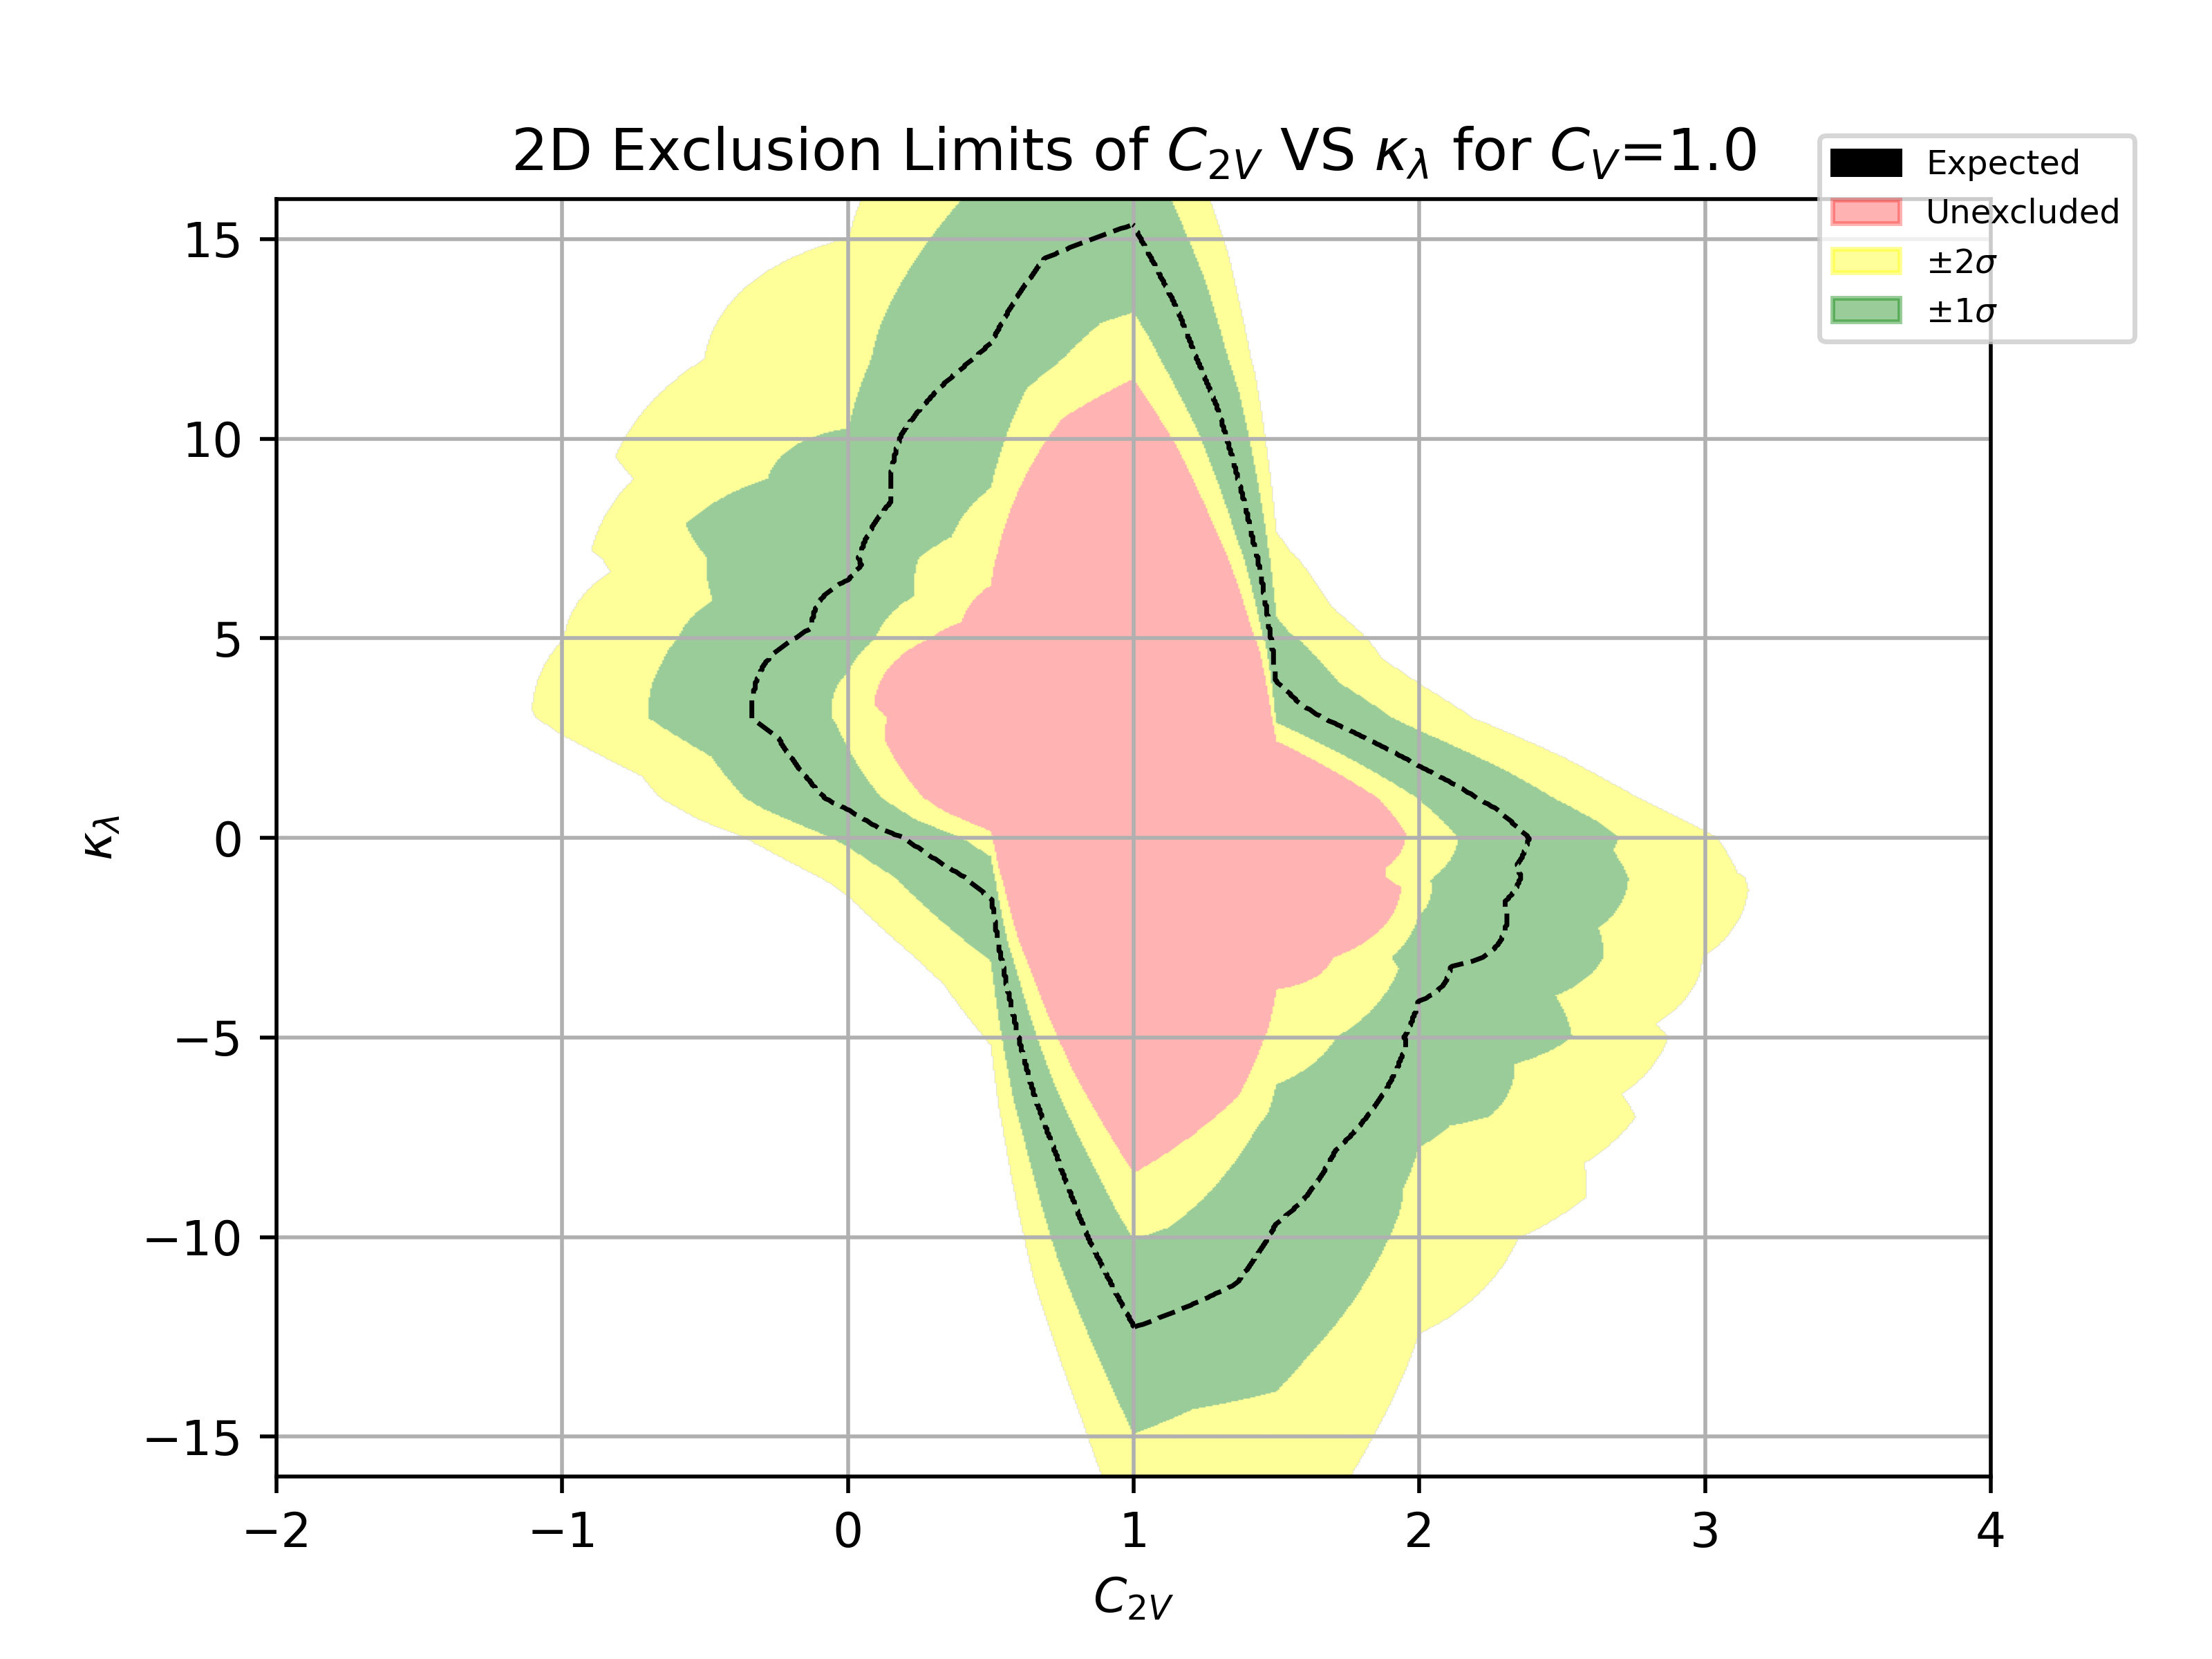
\includegraphics[width=\linewidth,height=0.8\textheight,keepaspectratio]{2D_scan_scan_test_beta5_samps_vbf_pd_161718_c1v1.0_exclusion}
        \end{column}
    \end{columns}
}

\fullscreenimage{Exclusion Across 3D Parameter Space}
{2D_scan_scan_test_beta5_samps_vbf_pd_161718_c1v_multislice_exclusion}

\fullscreenimage{Exclusion From a Different Perspective}
{2D_scan_scan_test_beta5_samps_vbf_pd_161718_kl_multislice_exclusion}
